\documentclass[12pt]{article}
\usepackage{graphicx}
\usepackage{float}
\usepackage{grffile}
\usepackage{color}
\usepackage{soul}
\usepackage{tabularx}
\usepackage{multirow}
% use \xspace to allow for space after a macro as necessary
\usepackage{xspace}
\usepackage[top=1in, bottom=1in, left=1.25in, right=1.25in]{geometry}
\usepackage{pdfpages}
%% maxwidth is the original width if it is less than linewidth
%% otherwise use linewidth (to make sure the graphics do not exceed the margin)
\makeatletter
\def\maxwidth{ %
  \ifdim\Gin@nat@width>\linewidth
    \linewidth
  \else
    \Gin@nat@width
  \fi
}
\makeatother

\definecolor{commentcol}{rgb}{0.345, 0.345, 0.945}
\newcommand{\comment}[1]{\textcolor{commentcol}{[[#1]]}}%

% general-purpose mathrm macros
\newcommand{\symsub}[2]{\ensuremath{#1_{\tiny \mathrm{#2}}}\xspace}
\newcommand{\mrm}[1]{\ensuremath{\mathrm{#1}}
\xspace}

\usepackage{framed}
\makeatletter
\newenvironment{kframe}{%
 \def\at@end@of@kframe{}%
 \ifinner\ifhmode%
  \def\at@end@of@kframe{\end{minipage}}%
  \begin{minipage}{\columnwidth}%
 \fi\fi%
 \def\FrameCommand##1{\hskip\@totalleftmargin \hskip-\fboxsep
 \colorbox{shadecolor}{##1}\hskip-\fboxsep
     % There is no \\@totalrightmargin, so:
     \hskip-\linewidth \hskip-\@totalleftmargin \hskip\columnwidth}%
 \MakeFramed {\advance\hsize-\width
   \@totalleftmargin\z@ \linewidth\hsize
   \@setminipage}}%
 {\par\unskip\endMakeFramed%
 \at@end@of@kframe}
\makeatother

\definecolor{randomcolor}{rgb}{.97, .27, .67}
\definecolor{shadecolor}{rgb}{.97, .97, .97}
\definecolor{messagecolor}{rgb}{0, 0, 0}
\definecolor{warningcolor}{rgb}{1, 0, 1}
\definecolor{errorcolor}{rgb}{1, 0, 0}
\newenvironment{knitrout}{}{} % an empty environment to be redefined in TeX

\usepackage{alltt}
\usepackage[sort]{natbib}
\usepackage{blkarray}
\usepackage{amsmath}
\usepackage{alltt}
\usepackage{hyperref}
\usepackage[utf8]{inputenc} % for accented characters
%% stuff for editing
%\usepackage[markup=nocolor,addedmarkup=bf,deletedmarkup=sout]{changes}
%% to suppress notes & comments: \usepackage[final]{changes}
\usepackage{setspace}
\usepackage{changes}
\usepackage[backgroundcolor=lightgray,textsize=tiny]{todonotes}

\bibliographystyle{chicago}
\title{Reformulating phylogenetic mixed models to improve flexibility and speed}
\author{Michael Li and Ben Bolker}
\date{\today}

\providecommand{\keywords}[1]{\textbf{\textit{Keywords:}} #1}
\IfFileExists{upquote.sty}{\usepackage{upquote}}{}
\begin{document}
\newcommand{\dbic}{\ensuremath \Delta \textrm{BIC}}

%% don't typeset BMB comments
\newcommand{\bmbhide}[1]{}
\newcommand{\bmb}[1]{{\color{blue} BB: #1}}

\newcommand{\fref}[1]{Figure~\ref{fig:#1}}

\newcommand{\mli}[1]{{\color{red} ML: #1}}

\newcommand{\add}[1]{{\color{blue} ADD: #1}}


%\SweaveOpts{concordance=TRUE}
%\SweaveOpts{concordance=TRUE}
\maketitle

\doublespacing

\keywords{phyloglmm, species--branch matrix, phylogenetic correlation, phylogenetic comparative methods}


\section*{Introduction}

Ever-increasing data collection capabilities (e.g. genomic sequencing, telemetry studies of animal behaviour, or environmental remote sensing), in combination with large-scale synthetic data bases of species occurrence and phenotypic traits, are making larger volumes of biological data available over an ever-wider taxonomic range.
Researchers use these data to fit complex models describing species occurrence and traits.
In particular, phylogenetic comparative methods (PCM) using phylogenetic (eco-evolutionary) regression \citep{hansen2012interpreting} is a powerful technique to explore relationships among species traits or distributions.
% \bmb{might be interesting to do some bibliometry, although absolutely not necessary --- i.e. how do numbers of citations of (whatever) increase relative to the overall size of the eco/evo literature? \ldots}
Given a known phylogenetic tree, PCMs explore the relationships among species traits or distributions while taking the underlying evolutionary relationships of the species into account; they can be used to control statistically for phylogenetic relationships, to quantify the phylogenetic signals (a measure of dependence among species responses due to their phylogenetic relationships) in trait distributions, or both.
Unlike standard statistical models, where all of the predictor variables of interest (for example, species traits and environmental factors) are directly observable,  PCMs use phylogenetic relationships to estimate the amount of unobserved process of trait evolution \citep{felsenstein1985phylogenies, butler2004phylogenetic}. 
% While evolutionary relationships are biologically important and interesting, they often get neglected in applications and multi-species analyses \citep{bunnefeld2012island, santamaria2012evolution}. 
Ecologists have used phylogenetic relationships in multi-species models \citep{garland1992procedures, freckleton2002phylogenetic, ord2010adaptation, davies2013phylogenetic}; and more recently becoming increasingly popular, they have begun to integrate evolutionary knowledge in applied ecological studies addressing biodiversity conservation and the effects of climate change \citep{winter2013phylogenetic, santamaria2012evolution, lankau2011incorporating, lavergne2010biodiversity, mace2008evolutionary}.
While a wide range of tools is available for comparative analyses, existing procedures may be either insufficiently flexible or too computationally demanding when analyzing large volumes of data.
In such cases, researchers must find ways to simplify their analyses: for example, treating species effects as independent, thus neglecting phylogenetic correlations among species responses \citep{bunnefeld2012island}; ignoring degrees of relatedness and treating taxon as a strictly hierarchical description \citep{tella1999habitat}; or neglecting within-species variation \citep{ord2010adaptation}.
%% bunnefeld2012island: used taxon for random slopes but did not include phylogenetic information
%% ord2010adaptation : used OU process with means (single obs per taxa),
%%  i.e. ignoring within-taxon variation?
%% fix me!?
% which can lead to statistical issues and erroneous conclusions
% \citep{felsenstein1985phylogenies, li2017statistical}.
% \bmb{What precise ``issues'' do you have in mind? Don't think we need to state them here, but we should know. Based on your comments, I can guess that (1) by using random slopes across taxa, Bunnefeld 2012 is neglecting more subtle variation due to differential relatedness? (2) not sure whether taking taxon-level means (Ord 2010) is actually a problem. Ignores some variation,
% but it might be ignorable (cf. Murtaugh 2007 ``Simplicity and complexity in ecological data analysis'')}
In this paper, we propose an alternative method for flexibly and efficiently modeling phylogenetic relationships via mixed effect models through random effects. 
This method allow researchers to easily incorporate various complexities without sacrificing speed.

\subsection*{Challenges in modeling phylogenetic process in multispecies data}

Multispecies data sets are often very challenging to model using basic statistical frameworks due to the complexity and non-normality data. 
Most researchers typically use basic regression based methods such as generalized-linear models (GLMs) and suffocated ecologist would use generalized-linear mixed effect models \citep{bolker2009generalized} to control for different levels of variation.
Most of the basic statistical techniques assume species are independent, which are false from a evolutionary perspective.
The classic phylogenetic regression uses a statistical model that is equivalent to assuming that phylogenetic correlation in the residuals from a regression between two species-level traits arises because the residual variation in the trait that is the dependent variable evolves along the branches of the phylogeny according to a Brownian-motion evolutionary model \citep{felsenstein1985phylogenies}. 
If the residuals are normally distributed and observed without any additional error or within-species variation, Felsenstein's method of phylogenetically independent contrasts (PICs) \citep{felsenstein1985phylogenies, nicolakakis2000forebrain} is sufficient to account for the phylogenetic correlation.
More recent approaches -- including phylogenetic generalized linear mixed models (PGLMM) \citep{ives2011generalized}, Pagel's $\lambda$ \citep{pagel1999inferring}, and Blomberg's $K$ \citep{blomberg2003testing} --- build upon PICs by considering different (non-Normal) response distributions and by accounting for additional complexities in the evolutionary process. 
In particular, these methods can partition residual variation into two components: (1) uncorrelated, or independent, residual variation (observation error or tip variation) and (2) phylogenetic signal  (biological/evolutionary process error) \citep{hansen2012interpreting}.
However, if each species' traits are observed more than once, possibly under different conditions, we can potentially distinguish third level of variation; in this case, phylogenetic signal and tip variation are now both part of the evolutionary process error (which we will call tip variation as intercept-level variation) while the among species residual error is associated with among observations variation within each species.
%\bmb{This is a good point, well expressed. Does PGLMM lump tip variation and within-species variation, or is this primarily an issue with Blomberg/Pagel? Thinking about Boettiger's critique \cite{boettiger2013is} (don't know if it's been peer-reviewed, we could ask him), which might be resolved if we think explicitly about within-species variation \ldots
%\mli{I think it is more like our simulation test. In Boettiger's example, it is treating sister taxa as different species. So it is using a phylogenetic tree of 8 species instead of 4.}
Although many studies include multiple observations per species, phylogenetic analyses rarely take advantage of such observations to partition variability more finely.
Indeed, many existing methods cannot accommodate multiple observations per species, instead requiring users to collapse the data by taking species averages.
Figure \ref{fig:variation} illustrates a visual categorization of various forms of variation for three species. 
%Despite having multiple observations per tip taxon (species), a typical part of observational or experimental design, but it is rarely seen: existing platforms are unable to fit multiple observations, or unbalanced design data, or both.
% \bmb{OK, but we should be prepared to support this. Could we construct a table of existing approaches/platforms with their capabilities?}

\begin{center}
\begin{figure}[H]
  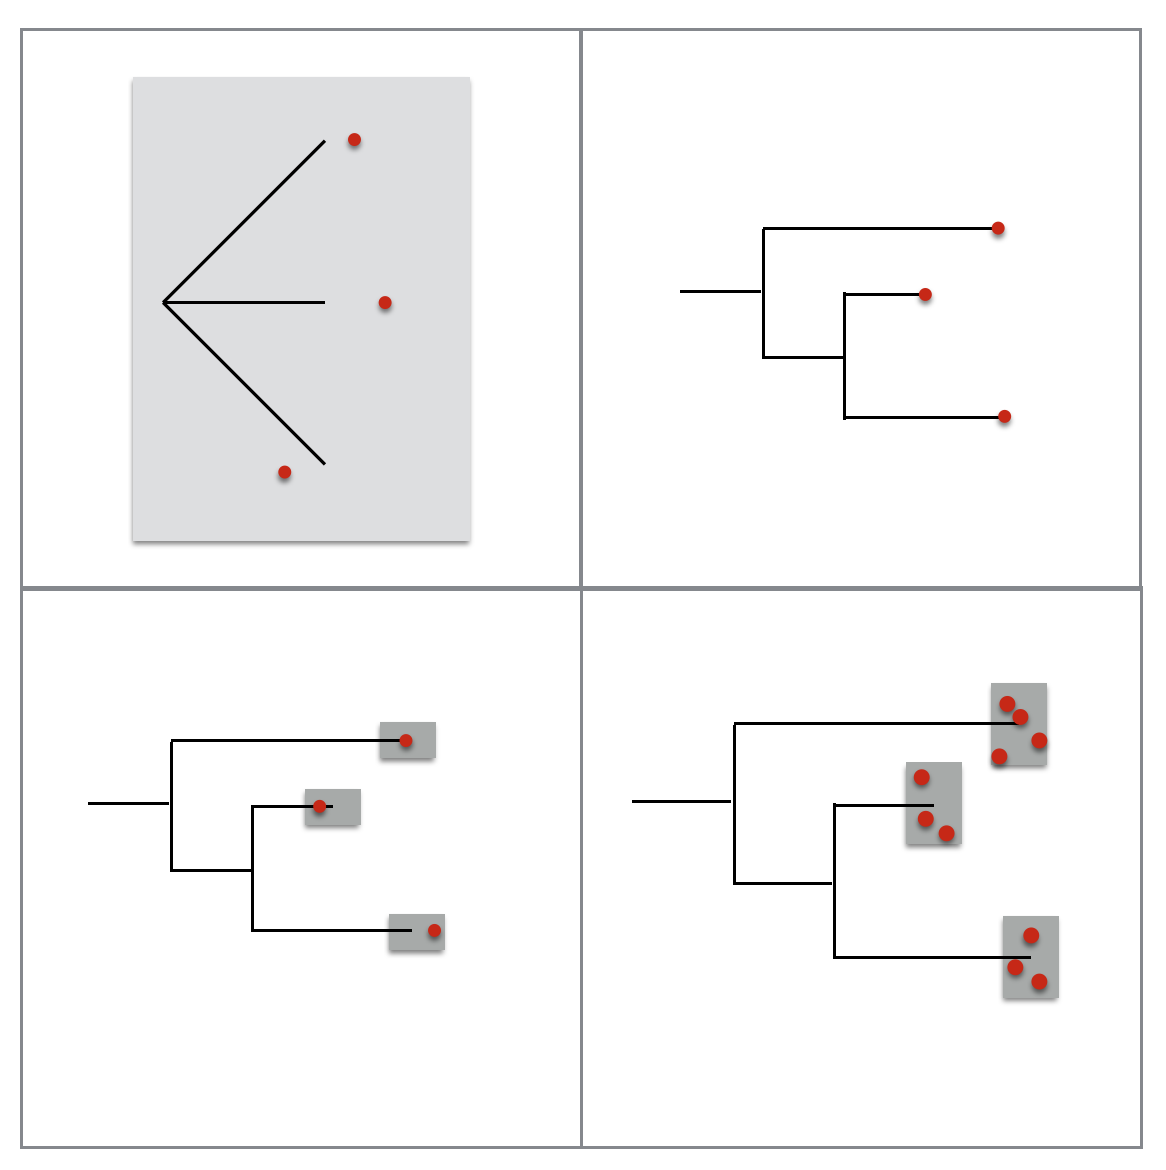
\includegraphics[scale=0.8]{./phylo_diagram.png}
  \caption{Visual categorization of various forms of phylogenetic variation of three species. Top left shows pure noise (i.e. assuming a star phylogeny); top right accounts for phylogeny, but without noise; bottom left accounts both phylogeny and noise at the tip, and finally bottom right shows multiple observations (with noise) at the tips.}
\label{fig:variation}
\end{figure}
\end{center}

Classic PCMs usually examines the response (trait or distribution) to vary according to the phylogenetic relationship across species, but it is plausible the changes in effect (or levels) of the predictor variables may vary according to the phylogenetic relationship across species as well.
Suppose we have exmained a collection of species that came from two groups, and wish to know whether their brain size (Y) is proportional to their body size (X) (Felsenstein's example \citep{felsenstein1985phylogenies}) using mixed-effect model. 
It is plausible that one group is simply larger than the other (random intercepts) with similar ratio, or alternatively, one group having a larger ratio (random slopes). 
%\bmb{maybe we can focus on random slopes here? Need to point out that example studies below are \emph{exceptions} to the general assumption of random intercepts only (how did they manage to do their inference?)}
Several recent studies have incorporated phylogenetic signals beyond species level and looked at species response to phylogenetic signals with changes in environmental factors.
For example, \cite{nowakowski2018phylogenetic} considered phylogenetically correlated slopes in response to habitat conversion when studying the abundance of amphibian species using a Bayesian implementation of phylogenetic GLMM, while \cite{li2017canfun} considered phylogenetically correlated species nested within sites for plant abundance via phylogenetic GLMM approach. 
The tools available for extending phylogenetic relationships to predictor variables (or predictor level variation) are relatively inflexible; thus, computationally sophisticated biologists have turned to more flexible Bayesian approaches, despite their computational burden \citep{hadfield2010mcmc, burkner2016brms}.
Table \ref{table:model} provides a summary of model complexities, platforms and data constraints for phylogenetic comparative analysis.

\newcommand{\pkg}[1]{{\tt #1}}
\newcommand{\code}[1]{{\tt #1}}

%% FIXME: chart looks ugly
\begin{table}[]
\begin{tabular}{|l|l|l|l|}
\hline
\textbf{Model}                                                                                    & \textbf{Method}                                                       & \textbf{Data}                                                                & \textbf{Platform}                                                                              \\ \hline
\multirow{2}{*}{\begin{tabular}[c]{@{}l@{}}Generalized Linear \\ Model (GLM)\end{tabular}}        & Correlated residual                                                   & Single Observation                                                           & \begin{tabular}[c]{@{}l@{}}\pkg{nlme}:gls, \\ \pkg{ape}:pic\end{tabular}                                   \\ \cline{2-4} 
                                                                                                  & \begin{tabular}[c]{@{}l@{}}Residual \\ + phylo intercept\end{tabular} & Single Observation                                                           & \begin{tabular}[c]{@{}l@{}}Pagel's $\lambda$\\ Blomberg's $k$ \\ via \pkg{nlme}:gls\\ \pkg{phylolm}\end{tabular} \\ \hline
\multirow{2}{*}{\begin{tabular}[c]{@{}l@{}}Generalized Linear \\ Mixed Model (GLMM)\end{tabular}} & \multirow{2}{*}{Random effect}                                        & \begin{tabular}[c]{@{}l@{}}Single Observation\\ Balanced Design\end{tabular} & \pkg{pez}                                                                                            \\ \cline{3-4} 
                                                                                                  &                                                                       & Unrestricted                                                                 & \pkg{lme4}, \pkg{glmmTMB}                                                                                  \\ \hline
\multirow{2}{*}{Bayesian GLMM}                                                                    & \multirow{2}{*}{Random effect}                                        & Balanced Design                                                              & \pkg{MCMCglmm}                                                                                       \\ \cline{3-4} 
                                                                                                  &                                                                       & Unrestricted                                                                 & \pkg{brms}                                                                                           \\ \hline
\end{tabular}
\caption{List of phylogenetic generalized linear models and R packages.}
\label{table:model}
\end{table}

In this paper, we will propose an alternative formulation of phylogenetic generalized linear mixed models that is mathematically equivalent to previous approaches, but more flexible.
Our new formulation can be incorporated in any framework that allows for random effect (such as random intercepts, slopes, and interactions) without the need to implement special correlation structures by incorporating phylogenetic structures as part of the mean model. 
%% can be incorporated relatively easily into any mixed-model platform that allows new random-effects design matrices to be specified, and can be easily extended along with the features of mixed model such as multiple observational designs, phylogenetic random-slopes models, and multiple (nested or crossed) random effects.
We will compare our technique coded in R package \pkg{lme4} and \pkg{glmmTMB} with existing R packages (i.e. \pkg{nlme} \citep{pinheiro2014r}, \pkg{phylolm} \citep{ho2014phylolm}, \pkg{pez} \citep{pearse2015pez} \pkg{phyr} (Li et al, unpublished), \pkg{MCMCglmm} \citep{hadfield2010mcmc}, and \pkg{brms} \citep{burkner2016brms}) fitting models to data from simulated model that incorporates phylogenetic signal from both predictors and tips/species, as well as residual variation.
As well as being flexible, we also expect that our approach will be fast, because \pkg{lme4} and \pkg{glmmTMB} use efficient approaches. 
%% FIXME: move to methods/simulations
% In principle, for any given valid method that matches the simulation model should eventually converge to the simulated parameters. 
% We end by discussing opportunities and practicalities of our method and comments on the state of art for this area of research. 

\section*{Materials and Methods}

\newcommand{\bX}{{\mathbf X}}
\newcommand{\bbeta}{{\boldsymbol \beta}}
\newcommand{\bmu}{{\boldsymbol \mu}}
\newcommand{\bY}{{\mathbf Y}}
\newcommand{\bC}{{\mathbf C}}
\newcommand{\bZ}{{\mathbf Z}}
\newcommand{\bb}{{\mathbf b}}
\newcommand{\besp}{{\boldsymbol \epsilon}}
\newcommand{\bSigma}{{\boldsymbol \Sigma}}

\subsection*{Phylogenetic regression}

We begin by describing the classic PCM in a linear regression setting.
Consider a simple linear regression model of observable trait $\bY$ as a function of some predictors $\bX$. 
The standard phylogenetic regression can be formulated as

%\bmb{boldface matrices/vectors i.e. $\bX \bbeta$? or not worth the trouble? How about $\bmu=\bX \bbeta$; $\bY \sim \textrm{MVN}(\bmu,\sigma^2 \bC)$ for greater generality? (OK, I see that you move in this direction later.  But I'm not sure it's worth the detour of using two different notations? even if you are going to extend to include fixed effects, $Z$, etc. later ...}:

\begin{align}
\bmu & = \bX \bbeta  \label{eq:gls1} \\ 
\bY & \sim \textrm{MVN}(\bmu,\sigma^{2} \bC), \label{eq:gls2}
\end{align}
where $\bX$ is an $n \times m$ model matrix, describing $n$ observations of $m$ predictor variables (phenotypic traits or environmental variables, typically including an intercept column of ones); $\bbeta$ is an $m$-vector of coefficients; $\bY$ is an $n \times 1$ response vector which is assumed to be multivariate normally distributed with mean $\bmu$ and variance-covariance matrix given by $\sigma^{2} \bC$ where $\bC$ is a $n \times n$ phylogenetic correlation matrix.
The PC matrix is inferred from the topology of the evolutionary tree by quantifying the degree of shared evolution between any pair of taxa \citep{garamszegi2014modern}.

%\bmb{give a ref for this? maybe Paradis's ape book, or Garamszegi's book, or ?}
%\mli{chapter 7 in garamszegi 2014}

% More recently, researchers use linear mixed model and generalized linear mixed model framework to model complex systems with phylogenetic structures.
%\mli{Why? Data type, interactions, random effects, etc... Need to really explain random effects here. Alternatively, we can drop this line and write this...}

\subsection*{Phylogenetic generalized linear mixed model}
Alternatively, one can use the generalized linear mixed effects modeling (GLMM) framework \citep{lynch1991methods}.
The generalized linear mixed effect model is an extension of the classic regression model, a kind of hierarchical linear model that can flexibly incorporate more than one kind of variability through random effects and for non-Gaussian responses.
The typical GLMM has the form:
\begin{align}
\bY & \sim \mathbf{f}(\bmu) + \besp \label{eq:glmm1} \\
\bmu & = \bX \bbeta + \bZ \bb  \label{eq:glmm2} \\
\bb & \sim \textrm{MVN}(0, \bSigma(\theta)) \label{eq:glmm3} \\
\besp & \sim \textrm{N}(0,\sigma^{2}_{\epsilon}) \label{eq:glmm4}
\end{align}
where $\bZ$ is an $n \times m$ model matrix for the $n$ -- dimensional vector-valued $m$ predictor variables; $\bb$ (sometimes referred as the "G-side" effect) represents the conditional modes and assumed to be multivariate normally distributed with a variance-covariance matrix given by $\bSigma(\theta)$; $\besp$ (sometimes referred as "R" effect) is an $n \times 1$ vector of independent and normally distributed error terms with variance $\sigma_{\epsilon}^2$.
Analogously, the phylogenetic regression given by (\ref{eq:gls1}) can be represented in the generalized mixed model framework with Gaussian responses by constraining $\bSigma(\theta) = \sigma^2 \bC$ and $\sigma^{2}_{\epsilon} = 0$.

There are several advantages in modeling phylogenetic correlated traits in the mixed model framework.
First, random intercepts can allow the response trait to vary across groups/levels within grouping predictors (e.g. patch, site, experiment, and etc). 
Second, it can also allow the response (trait or distribution) to vary according to the phylogenetic relationships across species (i.e. similar species will have similar responses), and between species (tip variation).
The third type of variation that is often neglected or rarely considered are random slopes.
Random slopes can allow fixed effects (size of the effect in continuous predictor variables) to vary for each species. 
Analogous to modeling the response dependency via phylogenetic relationship among species, phylogenetic random slopes can allow fixed effects to account for the phylogenetic relations (i.e. similar species will have similar size of the effects on the response than distinct pairs).


% \bmb{worth including the \pkg{MCMCglmm}/\pkg{brms} inverse-VCV formulation here? And/or contacting Eric Pedersen to find out about his Markov Random Field phylog. stuff in GAM?}
% \mli{inverse VCV for BLUP? an alternative way to find the inverse of the vcv(phy)}
% \mli{G vs R, PIC and simple variations (phylolm ...) uses R and no G}

\subsection*{Reformulating the phylogenetic covariance matrix}
% The standard problem of phylogenetic comparative methods is to analyze relationships among data where the observations are gathered from nodes (usually tips) of a phylogenetic tree.
% Phylogenetic independent contrasts is a generalization of the paired comparisons method where contrasts are taken for each bifurcation (nodes) in a phylogenetic tree. 
% Assuming that traits evolve independently in each lineage following speciation, then the trait divergences that occur at one node are independent of divergence at other nodes.  


\newcommand{\bS}{{\mathbf S}}
\newcommand{\bJ}{{\mathbf J}}
\newcommand{\bB}{{\mathbf B}}
\newcommand{\bBadj}{{\mathbf B}_{\mbox{\tiny adj}}}
\newcommand{\bomega}{{\boldsymbol \omega}}
\newcommand{\bell}{{\boldsymbol \ell}}
\newcommand{\e}{{ \epsilon}}

An alternative approach is to model the phylogenetic correlation as a \textit{Gaussian process}. 
In particular, suppose that the evolutionary process is a Brownian-motion, which means that evolution of a continuous trait evolve independently, following a standard Brownian-motion, along each branch of the phylogeny.
In this case, the phylogenetic variability of a particular species can be written as the sum of the variances of evolutionary changes that occurred on all of the branches in its history. 
Thus, modeling the evolutionary history of each species with a sequence of independent errors with species--branch matrix $\bS$, is equivalent to imposing a correlation $\bC$.
For example, for the phylogeny in figure \ref{fig:tree}, the corresponding $\bS$ takes the form:

%% FIXME: need top/side labels
\begin{center}
\begin{figure}[H]
  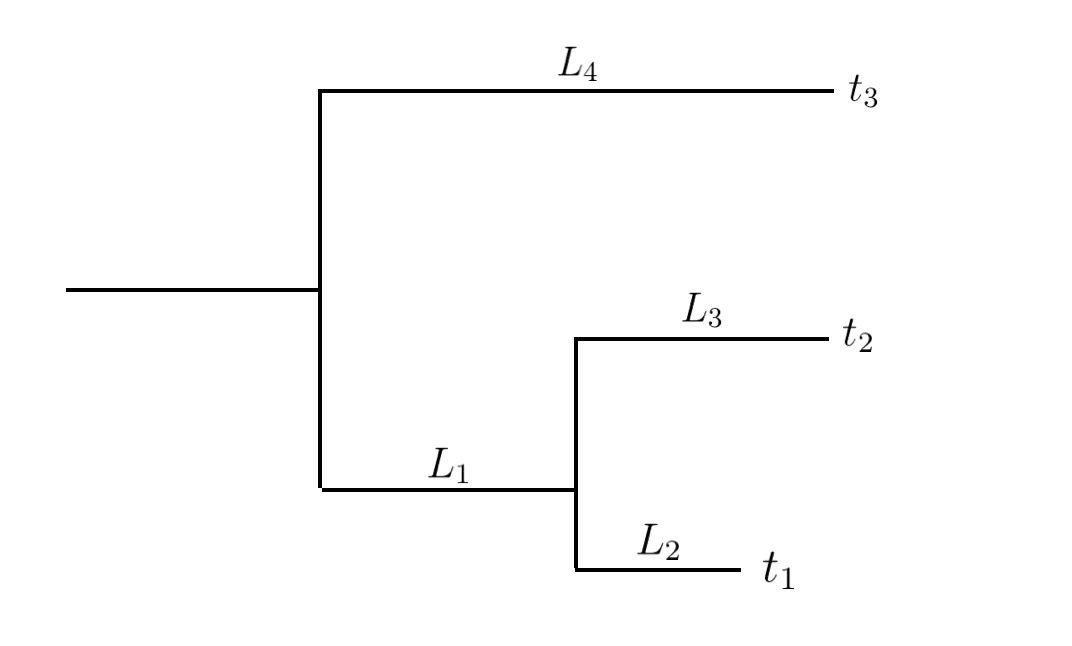
\includegraphics[scale=0.8,page=1]{./figure/phylotree.png}
  \caption{Three species phylogenetic tree.}
\label{fig:tree}
\end{figure}
\end{center}

\[
\begin{blockarray}{ccccc}
 & L_1 & L_2 & L_3 & L_4  \\
\begin{block}{c(cccc)}
  t_1 & \ell_1 \e_1 & \ell_2 \e_2 & 0           & 0 \\
  t_2 & \ell_1 \e_1 &  0          & \ell_3 \e_3 & 0 \\
  t_3 & 0           &  0          & 0           & \ell_4 \e_4 \\
\end{block}
\end{blockarray}
 \]

%% FIXME: double check this
The phylogenetic variability corresponding to species 1 is $\ell_1 \e_1 + \ell_2 \e_2$, where $\ell_i = \sqrt{L_i}$, the square root of the branch length $L_i$ in figure \ref{fig:tree} and the $\ell_i$ are independent, homoscedastic Normal variates with zero mean and $\sigma^2$ variance (i.e. the variance for species 1 is $(\ell_1 \e_1 + \ell_2 \e_2)^2 = (\ell_1^2 + \ell_2^2)\sigma^2$).
The variance of Brownian-motion, is the evolutionary rate, where it is linear in evolution time.

\subsubsection*{Constructing the species--branch random effects model matrix}

The $\bS$ matrix is the product of an $n \times b$ indicator matrix $\bS_{ind}$ of branch indices and $\bell$ is a vector of square root branch lengths.

\begin{align}
\bS_{ind} = \begin{bmatrix}
1 & 1 & 0 & 0 \\ 
1 & 0 & 1 & 0 \\ 
0 & 0 & 0 & 1
\end{bmatrix} , 
\qquad
\bell = \begin{bmatrix}
\ell_1 \\
\ell_2 \\
\ell_3 \\
\ell_4 
\end{bmatrix} .
\label{eq:S}
\end{align}
$\bS_{ind}$ is a binary (indicator) matrix that describes whether a particular branch occurs in the history of a focal species. 
$\bS \bS^T$ gives the variance-covariance matrix of the phylogeny. 

The random-effect model matrix $\bZ$ can be decomposed into term-wise model matrices $\bZ_{i}$ as described in \citet{bates2015fitting}.
Analogous to the procedure described in \citet{bates2015fitting}, the phylogenetic correlated random-effect matrix $\bZ^{C}_{i}$ is

\begin{equation}
\bZ^{C}_{i} = (\bS^{T}\bJ^{T}_{i} \ast \bX^{T}_{i})^{T}, \label{eq:ZC}
\end{equation}
where $\ast$ is the Khatri-Rao product \citep{khatri1968solutions}, $\bS$ is the $m \times b$ species--branch matrix; $\bJ_{i}$ is the $n_i \times m$ indicator matrix of grouping factors; and $\bX_{i}$ is the $n \times p_{i}$ raw random effects model matrix. 

For example, using the phylogeny above (figure \ref{fig:tree}), if we begin with a raw model matrix corresponding to a random-slope model, 

\begin{align}
\bX = \begin{bmatrix}
1 & t_1  \\ 
1 & t_2  \\ 
1 & t_3 
\end{bmatrix} 
\end{align}
then the term-wise phylogenetic random effects model matrix is,

\begin{align}
\bZ^{C}_{i} = (\bS^{T}_{adji}\bJ^{T}_{i} \ast \bX^{T}_{i})^{T} =
\left[
\left(
\begin{bmatrix}
\ell_{1} & \ell_{1}  & 0 \\
\ell_{2} &  0  & 0 \\
0  &  \ell_{3} & 0 \\
0 & 0 &  \ell_{4} 
\end{bmatrix}
\begin{bmatrix}
1 & 0  & 0 \\
0 & 1  & 0 \\
0 & 0  & 1  
\end{bmatrix}
\right)
\ast
\begin{bmatrix}
1   & 1   & 1  \\ 
t_1 & t_2 & t_3
\end{bmatrix} 
\right]^T
\\
= \begin{bmatrix}
\ell_{1} & \ell_{1}t_1 & \ell_{2} & \ell_{2}t_1 & 0 & 0 & 0 & 0 \\
\ell_{1} & \ell_{1}t_2 & 0 & 0 & \ell_{3} & \ell_{3}t_2 & 0 & 0 \\
0 & 0 & 0 & 0 & 0 & 0 & \ell_{4} & \ell_{4}t_3
\end{bmatrix}.
\end{align}


% 
% The scaled species--branch matrix $\bS_{adji}$ is scaled version of $\bS$ via the standardized generalized variance (SGV).
% SGVs are used as an intrinsic/natural way to scale down the variance-covariance matrix measured in different scales (for example, phylogenetic distance, years and etc) compariable to other variation in the model \citep{sengupta1987tests}.
% SGV is the $nth$ root of the generalized variance (GV), or the determinant of the variance-covariance matrix, where GV measures the overall size or volume of the variance-covariance matrix.  
% The SGV is given by:
% \begin{align}
% \bomega & = \textrm{det}(\bSigma_{phy})^{1/n},
% \end{align}
% where $n$ is the number of species in the phylogeny.
% 
% The analog in the $\bS$ is to scale the branch vector $\bell$ by square root of the SGV:
% \begin{align}
% \bell_{adj} & = \frac{\bell}{\sqrt{\bomega}}
% \end{align} 
% and the $\bS_{adj}$ is the matrix product of $\bS_{ind}$ and $\bell_{adj}$.

\subsection*{Simulation}
\subsubsection*{Single group model}

We generated test data based on the random slopes mixed model formulation (\ref{eq:glmm1}, \ref{eq:glmm2}, \ref{eq:glmm3}, \ref{eq:glmm4} ) with a single response variable $\bY$ and a single predictor continuous variable $\bX$ for $n$ = 25, 50, and 100 species.
For simplicity, the response variable $\bY$ is conditional normally distributed (i.e. Gaussian distribution with an identity link function) , which is a linear mixed effect model. 
For the first set of simulation, we simulate one observation per species.
% For wider range of comparisons, we simulate one observation ($X_i,Y_i$) per species.
The full simulation model is the following:
\begin{align}
\bY & = (\beta_0 + b_{\mathrm{phy_{int}}}) + (\beta_1 + b_{\mathrm{phy_{slope}}}) X + \besp  \label{eq:ss_sim}\\\
(b_{\mathrm{phy_{int}}}, b_{\mathrm{phy_{slope}}}) & \sim \textrm{MVN} \left( 0, \begin{bmatrix}
\sigma^2_{\mathrm{phy_{int}}} & \sigma_{\mathrm{phy_{int},phy_{slope}}} \\ 
\sigma_{\mathrm{phy_{int},phy_{slope}}} & \sigma^2_{\mathrm{phy_{slope}}}
\end{bmatrix} 
\right) \\ 
\besp & \sim \textrm{N} ( 0 , \sigma_{\epsilon}^2) .
\end{align}
The model contains two fixed effect parameters ($\beta_0$ and $\beta_1$), three random effect parameters (phylogenetic random intercept variance, phylogenetic random slope variance and covariance between phylogenetic random slope and intercept) and residual variance.  
The covariance between phylognetic random intercept and slope measures the correlation of phylogenetic dependency variability of the size in effect and outcome.
Predictor and intercept level random effect of species are not applicable in this simulation setting because there is no variation at the species level (i.e. single observation per species).

\subsubsection*{Multi-group model}

We extend the simulation model by adding multiple groups where each group has one observation per species. The multi-group full model is the following: 
\begin{align}
\bY & = (\beta_0 + b_{\mathrm{phy_{int}}} + b_{\mathrm{sp_{int}}} + b_{\mathrm{group}}) + (\beta_1 + b_{\mathrm{phy_{slope}}} + b_{\mathrm{sp_{slope}}}) X + b_{\mathrm{sp:group}} + \besp \label{eq:ms_sim}\\
(b_{\mathrm{phy_{int}}}, b_{\mathrm{phy_{slope}}}) & \sim \textrm{MVN} \left( 0, \begin{bmatrix}
\sigma^2_{\mathrm{phy_{int}}} & \sigma_{\mathrm{phy_{int},phy_{slope}}} \\ 
\sigma_{\mathrm{phy_{int},phy_{slope}}} & \sigma^2_{\mathrm{phy_{slope}}}
\end{bmatrix}
\right) \\
(b_{\mathrm{sp_{int}}}, b_{\mathrm{sp_{slope}}}) & \sim \textrm{MVN} \left( 0, \begin{bmatrix}
\sigma^2_{\mathrm{sp_{int}}} & \sigma_{\mathrm{sp_{int},sp_{slope}}} \\ 
\sigma_{\mathrm{sp_{int},sp_{slope}}} & \sigma^2_{\mathrm{sp_{slope}}}
\end{bmatrix}
\right) \\
b_{\mathrm{group}} & \sim \textrm{MVN} ( 0 , \Sigma_{\mathrm{group}}) \\
b_{\mathrm{sp:group}} & \sim \textrm{MVN} (0, \bf{I}_{\mathrm{group}} \otimes \sigma^2_{phy}) \\
\besp & \sim \textrm{N} ( 0 , \sigma_{\epsilon}^2),
\end{align}
where $\otimes$ is the Kronecker product.

The multi-group full simulation model has five additional random effects (predictor and intercept level random effect of species variance and their covariance, random intercept of group and random intercept of species-group interaction) compared to the single--group full model.
Predictor and intercept level random effect of species are now applicable in the multi-group model setting because there are multiple (one in each group) observations per species, thus there exist some form of variation at the species level.
Random intercept of species--group interactions describes whether the species within a group are more closely related on average than occurring by chance; which is equivalent to phylogenetic attraction as described in \cite{helmus2007separating}. 

\subsection*{Platforms}

Our algorithmic approach is general and could be implemented in a wide range of computational platforms that support independent latent variables as part of a linear or random effects (Z matrix) in generalized linear model. 
We implemented our approach using the R packages \pkg{lme4} \citep{bates2015fitting} and \pkg{glmmTMB} \citep{brooks2017glmmTMB}.
We compare our approach with five other R packages that can fit phylogenetic comparative models: \pkg{nlme} \citep{pinheiro2014r}, \pkg{phylolm} \citep{ho2014phylolm}, \pkg{pez} \citep{pearse2015pez}, and \pkg{brms} \citep{burkner2016brms}.
% \bmb{I think nlme can do other evolutionary models as well? May not be worth mentioning ...}
% \begin{verbatim}
% grep("\\.",apropos("^cor[A-Z]",ignore.case=FALSE),
% invert=TRUE,value=TRUE)
% \end{verbatim}
Phylogenetic generalized least squares (PGLS) (\code{gls} in \pkg{nlme}) is one of the most widely used techniques in phylogenetic comparative analysis; it simply fits a linear model where the covariance structure between species is equivalent to assuming a Brownian-motion evolutionary process (or other evolutionary process) on the tree instead of treating the residual variation as independent and identically distributed. 
Phylogenetic generalized linear models (PGLM) (\code{phyloglm} in \pkg{phylolm}) are a slightly more flexible variation of PGLS that can allow observational residuals and as well as non-Gaussian response variables.
Both packages can model other evolutionary processes and different correlation structures (i.e. Pagel's $\lambda$, Blomberg's $K$ etc.), but we restrict our PGLS fits to the simple BM correlation. 
Neither PGLS nor PGLM can handle multiple observations within a species or random slopes.
One of the few packages that currently fit phylogenetic correlations to predictor level variation is \pkg{pez} (and very recently \pkg{phyr}), which can handle adding additional uncorrelated random slopes and interactions with intercept.
Lastly, Bayesian phylogenetic GLMM using Markov chain Monte Carlo (MCMC) are available and can handle all of the cases described above. 
However, MCMC is often computationally expensive for GLMMs compared to platforms using deterministic optimization.
\pkg{MCMCglmm} \citep{hadfield2010general} is the most commonly used Bayesian phylogenetic GLMM, but we will instead use \pkg{brms}, which uses a more computationally efficient MCMC technique called Hamiltonian Monte Carlo (HMC) algorithm \citep{duane1987hybrid}.
 
% Table \mli{ref something} provides the statistically equivalent fitting capabilities of common/existing phylogenetic methods.
\begin{table}[]
\resizebox{\textwidth}{!}{%
\begin{tabular}{|c|c|c|c|c|c|c|}
\hline
\textbf{Package} & \pkg{nlme} & \pkg{phylolm} & \pkg{lme4}/\pkg{glmmTMB} & \pkg{pez} & \pkg{brms} & \pkg{MCMCglmm} \\ \hline
Single Group & X & X & X &  & X & X \\ \hline
\begin{tabular}[c]{@{}c@{}}Phylo Intercept\\ Phylo Slope\\ Phylo Slope-Intercept correlation\\ Residual\end{tabular} & X & \begin{tabular}[c]{@{}c@{}}X\\ \\ \\ X\end{tabular} & \begin{tabular}[c]{@{}c@{}}X\\ X\\ X\\ X\end{tabular} &  & \begin{tabular}[c]{@{}c@{}}X\\ X\\ X\\ X\end{tabular} & \begin{tabular}[c]{@{}c@{}}X\\ X\\ X\\ X\end{tabular} \\ \hline
Multi-group &  &  & X & X & X & X \\ \hline
\begin{tabular}[c]{@{}c@{}}Phylo Intercept\\ Phylo Slope\\ Phylo Slope-intercept correlation\\ Phylo Species-group interaction\\ Species intercept\\ Species Slope \\ Species Slope-intercept correlation\\ Residual\end{tabular} &  &  & \begin{tabular}[c]{@{}c@{}}X\\ X\\ X\\ X\\ X\\ X\\ X\\ X\end{tabular} & \begin{tabular}[c]{@{}c@{}}X\\ X\\ \\ X\\ X\\ X\\ \\ X\end{tabular} & \begin{tabular}[c]{@{}c@{}}X\\ X\\ X\\ X\\ X\\ X\\ X\\ X\end{tabular} & \begin{tabular}[c]{@{}c@{}}X\\ X\\ X\\ \\ X\\ X\\ X\\ X\end{tabular} \\ \hline
\end{tabular}%
}
\caption{List of estimable parameters for each R package.}
\label{table:platform}
\end{table}

\subsection*{Simulation and evaluations}
We simulated 100 phylogenetic trees for each sample size (n = 25,50,100 and additional n = 500 for multi-group model) and incorporated simulation parameters (illustrated in Figure \ref{ssplot} and Figure \ref{msplot}) to simulate responses from the simulation model (\ref{eq:ss_sim}, \ref{eq:ms_sim}).
Each realization were fitted to all model variant using different platforms.
Tables \ref{table:platform} shows the parameters that are estimable for each platform. 
We only evaluated the goodness of fit for model fits that passed the convergence tests implemented by the package.
For Bayesian GLMM, we combined two criteria to assess convergence: we required a value of the Gelman and Rubin statistic less than 1.1 and an effective sample size (ESS) greater than 1000 for the fixed effect parameters ($\beta_{0} \ \textrm{and} \ \beta_{1}$) for each replication. 
For each replication we sample two chains starting with 10000 iterations. 
%% TODO MAKE SURE THIS IS CORRECT!
We first evaluate our estimates by looking at the distribution of the estimated values (maximum likelihood estimates for non-Bayesian platforms and posterior medians for Bayesian platforms -- this gives us an idea of bias and variation (i.e. quality of the point estimate).
Then we look at frequentist coverage, to assess quality of confidence intervals.
Coverage refers to the frequency with which the computed confidence intervals include the true values of parameters.
We used 90\% (Wald and profile) confidence intervals and quantile-based intervals (for Bayesian GLMM) to evaluate coverage.
We also compare computational speed between different platforms to evaluate the efficiency of the platforms and methods. 

\section*{Results}

We used our method to reproduce the examples in [chapter 11] of \cite{garamszegi2014modern} using phylogenetic GLMMs based on `lme4` and `glmmTMB` (for more details see example in \cite{michael_li_2019_2639887}).
We also used our method and fitted the full model of the dune meadow data recently used with \pkg{pez} \citep{li2017canfun}. 
\pkg{lme4} and \pkg{pez} give identical results for fix and random effect estimates, our code is approximately 120 times faster than \pkg{pez}. 
Codes for fitting dune meadow analysis using \pkg{lme4} and \pkg{pez} are provided in the supplements. 

\subsection*{Single Group models simulations}

\begin{center}
\begin{figure}[H]
  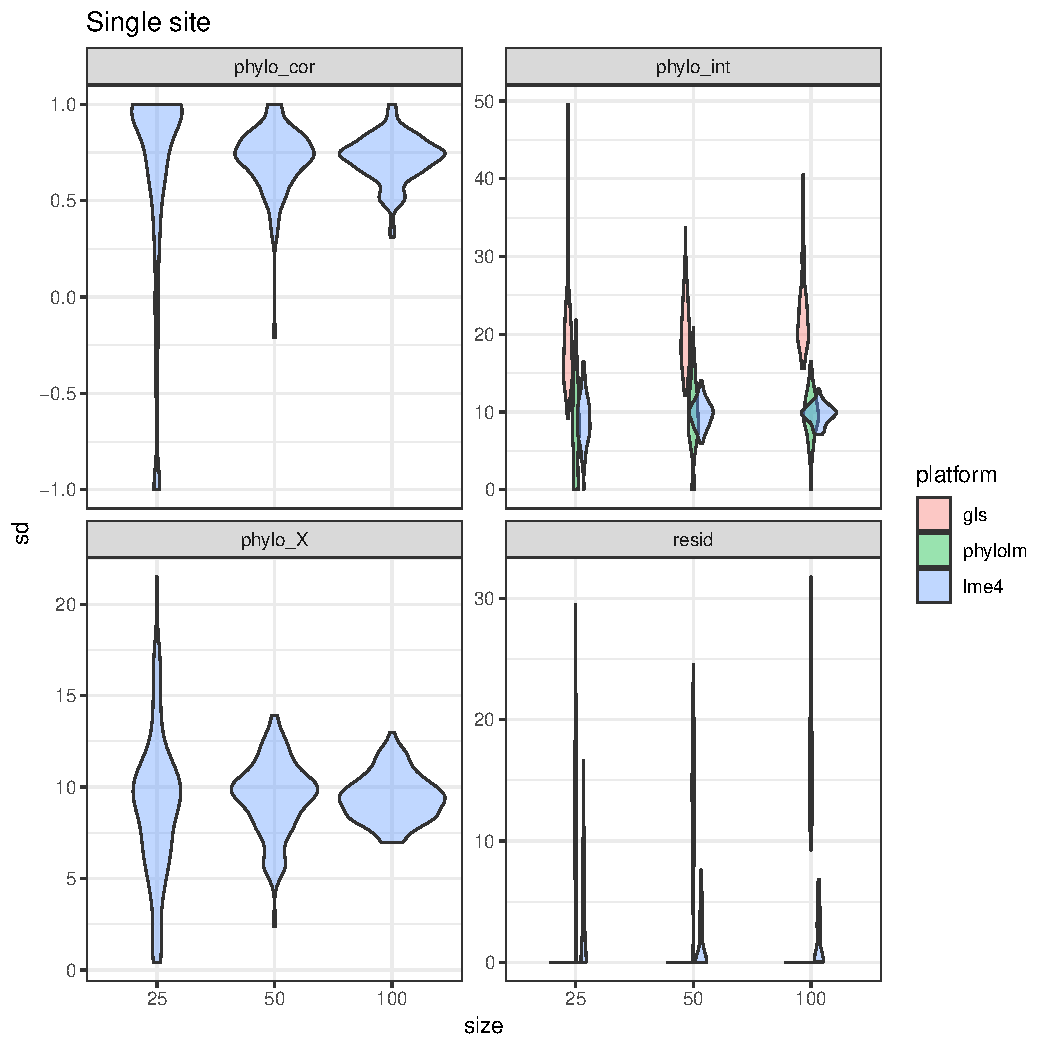
\includegraphics[scale=0.8,page=1]{./git_push/plot.Rout.pdf}
  \caption{Comparison of single group model parameter estimates across different R packages in Table \ref{table:platform}. The horizontal line shows the true value of the parameters in the simulation model. Models capable of fitting all parameters (\pkg{lme4}, \pkg{brms} and \pkg{glmmTMB}) fit well for all parameters.} 
\label{ssplot}
\end{figure}
\end{center}


\begin{center}
\begin{figure}[H]
  \includegraphics[scale=0.8,page=2]{./git_push/plot.Rout.pdf}
  \caption{Comparison of speed for all fitting packages variants: layout of the packages as in Figure \ref{ssplot}}
\label{ssplot_speed}
\end{figure}
\end{center}


\begin{center}
\begin{figure}[H]
  \includegraphics[scale=0.8,page=3]{./git_push/plot.Rout.pdf}
  \caption{Comparison of coverage probablility for fixed effect parameters. Models matching the simulation model (\pkg{lme4}, \pkg{brms} and \pkg{glmmTMB}) have coverage near the nominal value of 0.95. The black line shows the nominal coverage, and the grey ribbon the 95\% binomial confidence interval based on 100 simulated fits.}
\label{ssplot_coverage}
\end{figure}
\end{center}

The full fitted model (which matches the simulation model that incorporates phylogenetic intercept, slope and correlation) provides estimates with low bias (the difference between the parameter estimates and true simulation parameters) and variance for all parameters. 
Estimates for fixed effect parameters ($\beta_0$ and $\beta_1$) approach nominal coverage as the number of species increases for \pkg{lme4} and \pkg{glmmTMB} but not for other packages. \pkg{brms} have higher coverage than the nominal coverage at 95 \% because the prior distributions for the simulation parameters are cenetered at the true values.
%% \mli{Is there a figure for this?....Ok, maybe We don't need it.}

In general, models that are insufficiently flexible to match the true simulation model (PGLM and PGLS) will try to fit the data with the parameters available. 
PGLM (which lacks the phylogenetic slope parameter) provides reasonably good estimates for phylogenetic intercept parameter ($\sigma_{\mathrm{phy_{int}}}$) but overestimates the residual standard deviation; the estimates for the intercept ($\beta_0$) are slightly conservative (90\% coverage of the 95\% CI with 100 species) and the fixed slope parameter ($\beta_1$) have poor coverage ($<$ 60\%).
PGLS, with only one parameter available, confounds all variation (phylogenetic intercept, slope and residual variation) into the phylogenetic intercept parameter, resulting in overestimating the phylogenetic intercept and over-covering for $\beta_0$, and under-covering for $\beta_1$.

\subsection*{Multi-group model simulations}

\begin{center}
\begin{figure}[H]
  \includegraphics[scale=0.8,page=4]{./git_push/plot.Rout.pdf}
  \caption{Comparison of multi-group model parameter estimates across different R packages in Table 2. Annotations as in Figure \ref{ssplot}.}
  \label{msplot}
\end{figure}
\end{center}


\begin{center}
\begin{figure}[H]
  \includegraphics[scale=0.8,page=5]{./git_push/plot.Rout.pdf}
  \caption{Comparison of multi-group model computational speed across different R packages in Table 2. Annotations as in Figure \ref{ssplot}.}
  \label{msplot_time}
\end{figure}
\end{center}


\begin{center}
\begin{figure}[H]
  \includegraphics[scale=0.8,page=6]{./git_push/plot.Rout.pdf}
  \caption{Comparison of multi-group model coverage across different R packages in Table 2. Annotations as in Figure \ref{ssplot}.}
  \label{msplot_coverage}
\end{figure}
\end{center}


Multi-group model fits on the other hand, are much more similar across platforms (only the more powerful subset of platforms can fit these models at all, and the fitting models are closer to the true simulation model).
Similar to the single group fits, \pkg{lme4} and \pkg{glmmTMB} match the simulation model provides and good estimates for all parameters except the correlation ($\sigma_{\mathrm{sp_{int,slope}}}$) for few number of species (i.e. n = 25 and 50).
The lack of correlations in \pkg{pez} and \pkg{phyr}'s statistical models does not appear to have a large effect on the estimates of the remaining parameters in the model, whereas \pkg{pez} underestimates many parameters.  

Although the parameter estimates are similar across platforms for the multi-group simulation fits, computational efficiency varies enormously across platforms and sample size.
For example, the new formulation is implemented in both \pkg{lme4} and \pkg{glmmTMB}, but \pkg{glmmTMB} is almost an order of magnitude faster than \pkg{lme4}.
Comparing \pkg{glmmTMB} to \pkg{pez} and \pkg{phyr}, the median time for \pkg{glmmTMB} to fit 50 (100) species model takes $\approx$ 9 (20) versus $\approx$ 200 (2000) seconds for \pkg{pez} and \pkg{phyr}. 
\pkg{glmmTMB} takes $\approx$ 125 seconds to fit a 500-species model; it was not practical for \pkg{pez} and \pkg{phyr} to fit 500-species for our study, where the computational speed did not scale linearly with sample size 25/50/100.
\pkg{glmmTMB} is almost an order of magnitude faster than \pkg{lme4}.

% \bmb{Can you put a lower bound on \pkg{pez}'s computation time? How long did you take to give up? How does it scale? can you either figure out from first principles
%   or (easier) do a brute-force series of increasing sample size and
%   compute a log-log regression of time vs sample size to find the
%   approximate power?}

\newpage

\section*{Discussion}


% \bmb{say something about the implications of this [e.g. good enough for getting an overall impression of phylog. whatever-it-is but not enough for detailed description/inference about the evolutionary process?] (or maybe that should be saved for the Discussion?)}

The simulations presented in this paper are an oversimplification of the real evolutionary processes in nature, but they are no simpler than what researchers typically use.
In fact, our results showed that even simple single predictor--response multi-species model can incorporate multiple levels of complexity (e.g. including random slopes, intercept-slope correlations, and the phylogenetic analog) and fitting simpler variations can lead to wrong unreliable estimates of the fixed effects, which is typically the main point of interest.

We have fitted models using different platforms that best match the simulation models. 
Models that cannot match the simulation (full) model are expected to perform poorly; it is important to understand the limitations and performance of these simpler models that are restricted by the commonly used methods available.
Using models that include some form of phylogenetic variation and residual variation is necessary to detect and account for correlations between species via evolutionary processes.
Here are a few points researchers should think about when fitting phylogenetic regression models.

\subsection*{Process and observation variability and confounding}

% \bmb{explain: classical scenario for PIC is when we have species-level data (i.e., species averages or ``typical'' values).  What do we do when we have multiple observations per species?  Why can't we just average? (cf. \cite{murtaugh2007simplicity}) with a nested, balanced design, averaging by group and doing 1-way ANOVA gets the same answer for fixed effects as LMMs). \textbf{answers}: (1) unbalanced data (can handle by weighting by $n$, equivalent to assuming homoscedasticity and using inverse-variance weights); (2) non-Gaussian responses (averaging doesn't make sense) [can we use offsets to handle this case? don't know]; (3) maybe for equivalent of randomized block designs? (4) when within-species variance is actually of interest}
Process and observation errors are highly confounded in phylogenetic regression if it is not handled correctly. 
For single measurement per species model, any method that can account for at least two sources of variation (one for the residual variance, and at least one for the process variation) will be sufficient to a first approximation (i.e. Pagel's $\lambda$, Blomberg's $K$).
If multiple observations are allowed per species, then using methods such as Pagel's $\lambda$ can potentially incorrectly estimate the amount of phylogenetic process by substituting tip variation with residual variation, which is equilvent to Felsenstein's ``worst case".
There are a few ways to deal with this case.
For balanced data one can summarize multiple observations to a single measurement (for example, mean or median) per species to avoid confounding residual and tip variations.
For unbalanced data, one can handle by weighting by number of observations per species, which is equivalent to assuming homoscedasticity using inverse-variance weights. 
Alternatively, when within-species variance is actually of interest, accounting for within-species variance (i.e. adding species-level random effect in our example) can automatically handle multiple observations per species.

\subsection*{Random effects}

% \bmb{I think you need a lot more here; what does a random slopes model mean? You have one sentence that says ``people should be thinking about random slopes''. Then you talk about correlation (which is a much more subtle/less important issue, I think).}

In classic GLMM, random effects are often used to handle group (or individual) level variations by allowing for group effects. 
Random intercepts are often the ``go-to" method to handle these effects because it is controlling the group effects in the reponses level (i.e. the interest is the expected value of the response when all predictors are zero/unpresent) by allowing different intercepts.
Alternatively, random effects can be in more complicated forms such as random slopes (i.e. allow fixed effects to vary for each group), and they are much harder to interpret and think about in practice.
Random slopes models are not always appropriate, but they are relevant over a wider range of scenarios than people are currently thinking about \cite{schielzeth2008conclusions, cleasby2015quantifying,ord2010adaptation}.
Neglecting random slopes can lead to erroneous fixed effect estimates \citep{schielzeth2008conclusions} (parameters of interest) as shown in the simulations above. 
When analyzing relationships among species between traits, it is entirely plausible that change in effect of predictor variables have on traits are changing with respect to different grouping of species or even in phylogenetically correlated way (phylogenetic random slopes).
Nevertheless, it is hard to account for all forms of complexities and decide if phylogenetic random intercepts are more approriate than random slopes, or including both of them in the model.
It may be easier to be conservative to include both of them but simplify the phylogenetic relationships (at the random slopes level) and think about the random-slopes model in a strictly hierarchical setting (i.e., estimating different slopes for each family, or taxon \citep{bunnefeld2012island}) - the PGLMM collapses to a standard random-slopes model. 
Users should be aware of two important questions when fitting random-slope models: How much data do we need in order to practically estimate the random slopes? and Are we making a mistake by ignoring random slopes \citep{schielzeth2008conclusions}? 
% However, in the PGLMM context, as long as there's variation in the predictor among tips, there will be variation among taxa at some level, so random-slopes models will (almost always) be \emph{theoretically} identifiable.


\subsection*{Extension and alternatives}

Our analysis covers the classical phylogenetic comparative methods (i.e. phylogenetic least squares, linear and mixed models).
Even within the scope there is additional room for exploration we neglected, such as exploring phylogenetic multivariate response models, non-BM evolution processes (such as Ornstein-Uhlenbeck (OU) process which accounts for both selection and drift processes \cite{butler2004phylogenetic}), Bayesian approaches \cite{hadfield2010general}.
More broadly, the simple independence error approach we developed here offers a more efficient and mathematical equivalent way to do Brownian motion evolution process phylogenetic comparative analysis. 
This approach can in principle be combined flexibly with the state of the art phylogenetic mixed models using platforms that supports independent latent variables such as \pkg{MCMCglmm} \citep{hadfield2010mcmc}; a widely used Bayesian approach to PGLMM.
However, in principle just like GLMM and most statistically models, users should be aware the amount of data they have and the complexity of the model they want to fit (i.e. What should we do when we don't have enough data? Should we use a complex model and overfit \citep{barr2013random}, the right balance of complexity and data \citep{baayen2008mixed} or possibility of Bayesian approaches \cite{hadfield2010mcmc}).
More importantly, this implementation in \pkg{lme4} allows users to fit phylogenetic mixed models to the fullest ( that other frequentist platforms lack of (i.e. large data, unbalanced species observations, complex random effects) and explore new ideas.


\section*{Conclusion}

We have presented a simple approach to fit phylogenetic mixed models that is both more efficient and statistically equivalent approach and comparison of classical PCM to simulated data. 
First, this new approach is magnitudes faster compared to existing phylogenetic mixed models without losing robustness/accuracy and can easily combined with any statistically mixed model framework. 
Last and most importantly, it is more flexible in fitting large phylogenies, large volume of data, unbalanced data sets, and complex random effects such as slope correlations.

\newpage

\section*{Supplements -- translation}

$1 \mid Sp_{phylo}$, $0 + X_{E} \mid Sp_{phylo}$ and $X_{E} \mid Sp_{phylo}$ means phylogenetically related have similar response,   

\begin{tabularx}{\textwidth}{|l|X|X|}
\hline
Formula & Statistics & Biology \\
\hline
$1 \mid Sp$ &
random species intercept; variation within species in mean response across all factors &
variation of how species respond \\
\hline

$0 + X_{E} \mid Sp$ &
random slope of environment factor within species; variation in coefficient within species for the environmental factor &
variation of how species respond to the same environmental factor \\
\hline

$1 + X_{E} \mid Sp$ &
random slope of environmental factor within species with correlated intercept; variation in coefficient within species for the environmental factor with correlated mean response across all other factors &
variation of how species respond in the same environmental factors and the correlation of the variation of how they respond in general \\
\hline

$1 \mid Site:Sp $ &
random variation in intercept among species within sites &
variation of how species respond within sites \\
\hline

$1 | Sp_{Phylo} $ &
variation among species in mean response across all factors demonstrate phylogenetic signal &
phylogenetically related species respond similarly \\
\hline

$0 + X_{E} \mid Sp_{Phylo}$ &
variation among species for environmental factors demonstrate phylogenetic signal &
phylogenetically related species respond similar (share common response) to the same environmental factor \\
\hline
\end{tabularx}
            
            
            
            
            
                                                              


\bibliography{phyloglmm}

\end{document}

